\chapter{ダウンサンプリング}
    \section{ダウンサンプリングされた信号のDTFT}
        \newcommand{\xd}{x_\text{d}}
        \newcommand{\yd}{y_\text{d}}
        \newcommand{\Xd}{X_\text{d}}
        \newcommand{\Yd}{Y_\text{d}}
        \subsection{主張}
            記号を次のように定義する。
            \begin{itemize}
                \item $R\in\naturalNumbers,\;R\geq 2$ : ダウンサンプリングレート
                \item $\xd:\integers\to\complexNumbers$ : 離散時間信号
                \item $\Ts>0$ : $\xd$ のサンプル周期
                \item $\yd$ : $\xd$ を $1/R$ にダウンサンプリングした離散時間信号。つまり $\yd(n) = \xd(nR)$ 。
                \item $\Xd$ : $\xd$ のDTFT
                \item $\Yd$ : $\yd$ のDTFT
            \end{itemize}
            このとき $Y$ は次式で表される。
            \[ \Yd(\omega) = \frac{1}{R}\integrate{-\pi/\Ts}{\pi/\Ts}{\Xd(\tilde{\omega})\sum_{n=-\infty}^\infty\delta\parens*{\tilde{\omega}-\omega-n\frac{2\pi}{R\Ts}}}{}{\tilde{\omega}} \]
            $\Yd$ は $\omega$ に関する $2\pi/(R\Ts)$ 周期関数である。
            このことは $\omega$ に $2\pi/(R\Ts)$ の整数倍を加えてみれば容易に解る。
            $\Yd$ の第1 Nyquist 領域は $S_{\text{N},Y} \coloneqq [-\pi/(R\Ts),-\pi/(R\Ts))$ となる。
            \par
            $\Xd$ の台のうち $\xd$ の第1 Nyquist 領域 $S_{\text{N},X} \coloneq [-\pi/\Ts, \pi/\Ts)$ にある部分を $S_X$ とする。
            エイリアシングが生じない必要十分条件は $S_X\subset S_{\text{N},X}$ である。
            ここで言うエイリアシングとは、$S_X$ を $2\pi/(R\Ts)$ の整数倍ずつ平行移動しながら無限に複製したものを考えたとき、複製された $S_X$ 同士に重なりが生じることを指す。
        \subsection{導出}
            \begin{align*}
                \Yd(\omega) &= \sum_{n=-\infty}^\infty \yd(n)\exp(-i\omega nR\Ts) = \sum_{n=-\infty}^\infty \xd(nR)\exp(-i\omega nR\Ts) \\
                &= \sum_{n=-\infty}^\infty \IDTFTwithArg{\Xd}{nR}\exp(-i\omega nR\Ts) \\
                &= \sum_{n=-\infty}^\infty \parens*{\frac{\Ts}{2\pi}\integrate{-\pi/\Ts}{\pi/\Ts}{\Xd(\tilde{\omega})\exp\parens*{i\tilde{\omega}nR\Ts}}{}{\tilde{\omega}}}\exp(-i\omega nR\Ts) \\
                &= \frac{\Ts}{2\pi}\integrate{-\pi/\Ts}{\pi/\Ts}{\Xd(\tilde{\omega})\parens*{\sum_{n=-\infty}^\infty\exp\parens*{i(\tilde{\omega}-\omega)nR\Ts}}}{}{\tilde{\omega}} \\
                &= \frac{\Ts}{2\pi}\integrate{-\pi/\Ts}{\pi/\Ts}{\Xd(\tilde{\omega})\parens*{\frac{2\pi}{R\Ts}\sum_{n=-\infty}^\infty\delta\parens*{\tilde{\omega}-\omega-n\frac{2\pi}{R\Ts}}}}{}{\tilde{\omega}} \quad (\text{\ref{定数関数1のDTFT}を用いた。}) \\
                &= \frac{1}{R}\integrate{-\pi/\Ts}{\pi/\Ts}{\Xd(\tilde{\omega})\sum_{n=-\infty}^\infty\delta\parens*{\tilde{\omega}-\omega-n\frac{2\pi}{R\Ts}}}{}{\tilde{\omega}}
            \end{align*}
            被積分関数の $\Xd$ とデルタ関数列を次の図に示す。
            $\omega$ がデルタ関数列の原点からのオフセットである。
            \begin{figure}[H]
                \centering
                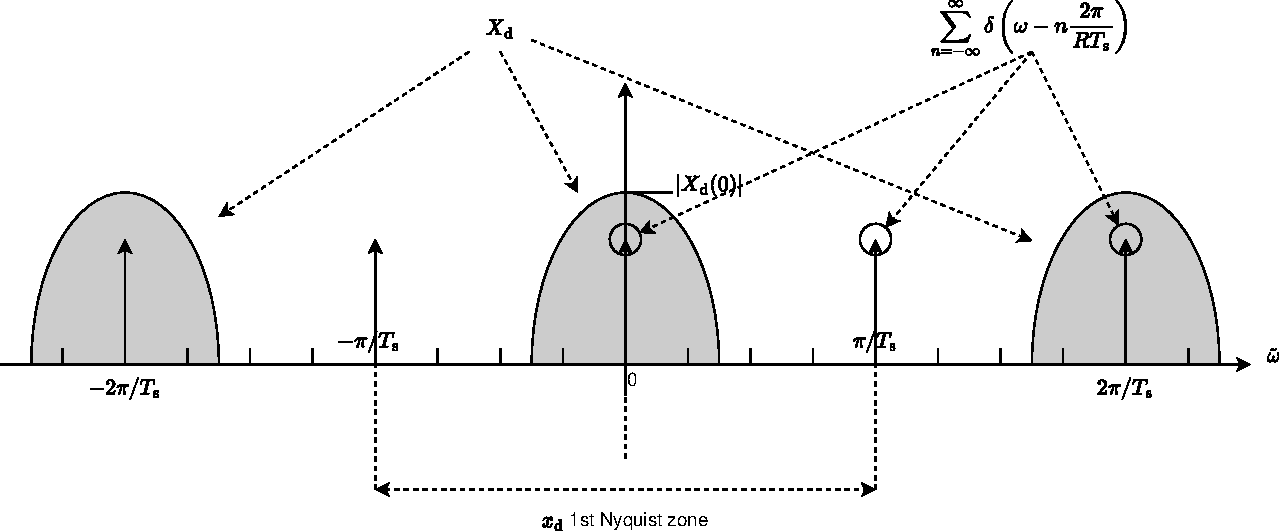
\includegraphics[keepaspectratio, scale=0.7]
                {\currfiledir/imgs/X_d_and_delta_impulse_series.pdf}
                \caption{$\Xd$ とデルタ関数列($R=2$)}
            \end{figure}
            エイリアシングが生じないことと $S_X \subset S_{N,\text{X}}$ が同値であることが解る。
            $\Yd$ を次の図に示す。
            \begin{figure}[H]
                \centering
                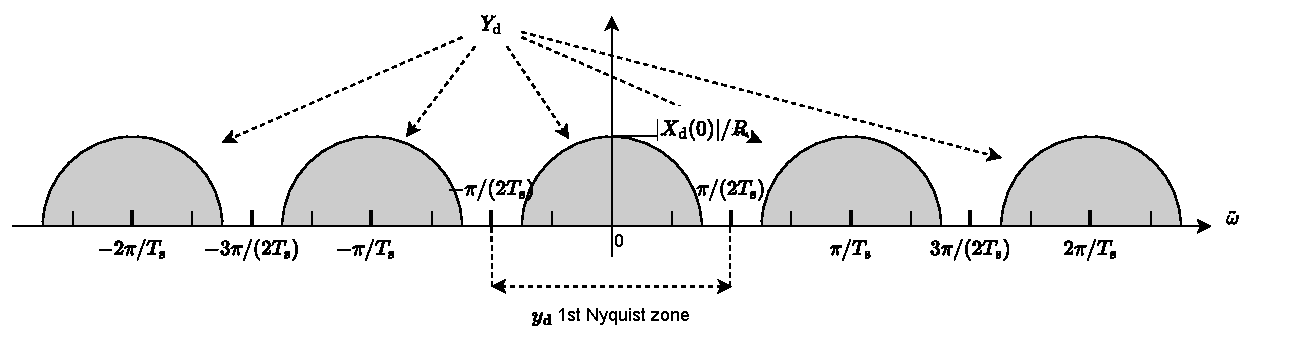
\includegraphics[keepaspectratio, scale=0.7]
                {\currfiledir/imgs/Yd.pdf}
                \caption{$\Yd$}
            \end{figure}
        \subsection{数値例}
            $x(t) = A\exp(-t^2/(2\sigma^2))$ のときの数値例が下記の Mathematica ノートブックにある。 \\
            \verb|DTFT_of_down-sampled_signal.nb|
